% Source: graduate-coursework/Sp26/CSCE775/HW1/HW1_CSCE_775_solutions.tex

\documentclass[border=4pt]{standalone}
\usepackage{amsmath}
\usepackage{amssymb}
\usepackage{bm}
\usepackage{graphicx}
\usepackage{pgfplots}
\usepackage{tikz}
\usepackage{xcolor}
\pgfplotsset{compat=1.18}
\usetikzlibrary{shapes.geometric, arrows.meta, positioning, automata, calc, decorations.markings, patterns}

\definecolor{USC_Garnet}{HTML}{73000A}
\definecolor{USC_Sandstorm}{HTML}{FFF2E3}
\definecolor{USC_Black90}{HTML}{363636}
\definecolor{USC_Black70}{HTML}{5C5C5C}
\definecolor{USC_Black50}{HTML}{A2A2A2}
\definecolor{USC_Black10}{HTML}{ECECEC}
\definecolor{USC_Honeycomb}{HTML}{A49137}
\definecolor{USC_Horseshoe}{HTML}{65780B}
\definecolor{USC_Atlantic}{HTML}{466A9F}
\definecolor{USC_Congaree}{HTML}{1F414D}
\definecolor{USC_Rose}{HTML}{CC2E40}


\begin{document}
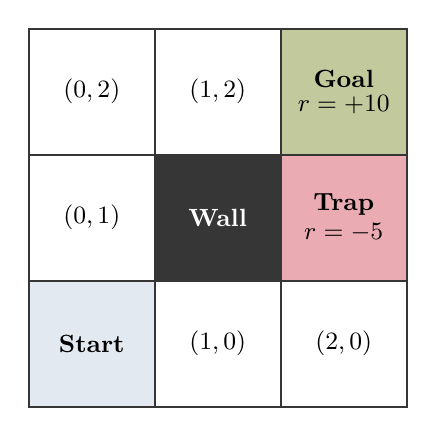
\begin{tikzpicture}[
    cell/.style={minimum size=1.6cm, draw=USC_Black90, line width=0.8pt, font=\small, anchor=center}
]

\node[cell, fill=white] at (0, 3.2) {$(0,2)$};
\node[cell, fill=white] at (1.6, 3.2) {$(1,2)$};
\node[cell, fill=USC_Horseshoe!40, font=\small\bfseries] at (3.2, 3.2) {\shortstack{Goal\\$r=+10$}};

\node[cell, fill=white] at (0, 1.6) {$(0,1)$};
\node[cell, fill=USC_Black90, text=white, font=\small\bfseries] at (1.6, 1.6) {Wall};
\node[cell, fill=USC_Rose!40, font=\small\bfseries] at (3.2, 1.6) {\shortstack{Trap\\$r=-5$}};

\node[cell, fill=USC_Atlantic!15, font=\small\bfseries] at (0, 0) {Start};
\node[cell, fill=white] at (1.6, 0) {$(1,0)$};
\node[cell, fill=white] at (3.2, 0) {$(2,0)$};

\end{tikzpicture}
\end{document}
